
\chapter{Large Language Models}

\section{LLM Network as Sequence-to-Sequence Machines via Transformer Models}

At their core, Large Language Models (LLMs) are sequence-to-sequence machines that generate a response sequence given an input sequence of words, converted into tokens. However, the way they process and generate these sequences involves several layers of complexity:

\begin{enumerate}
    \item \textbf{Contextual Understanding via Self-Attention} \\
    Unlike simple sequence models (e.g., RNNs), Transformers use self-attention to consider all tokens in a sequence simultaneously. This allows them to capture dependencies across long contexts.

    \item \textbf{Probability-Based Token Generation} \\
    At each step, the model predicts the next token by computing a probability distribution over the vocabulary. The output sequence is formed by sampling or selecting the most probable token at each step.

    \item \textbf{Task-Specific Adaptations}
    \begin{itemize}
        \item \textbf{Text Generation} (GPT, LLaMA, Mistral): Autoregressive models predict one token at a time, conditioning each step on previous outputs.
        \item \textbf{Text Understanding} (BERT): Masked language models predict missing tokens given bidirectional context.
        \item \textbf{Instruction-Tuned Models} (ChatGPT, Claude): Fine-tuned on dialogue and instruction-following data, allowing multi-turn interactions.
    \end{itemize}
\end{enumerate}

So, while LLMs fundamentally map an input sequence to an output sequence, their real power comes from how they encode context, manage dependencies, and adapt to various tasks through fine-tuning and prompting.

Large Language Models (LLMs) have revolutionized natural language processing (NLP) through the use of Transformer architectures. Introduced by Vaswani et al. in 2017, Transformers have surpassed previous recurrent and convolutional models in both efficiency and scalability. Let us give a quick overview of Transformer architectures and their role in modern LLMs.

The Transformer model is based on the self-attention mechanism and is composed of an encoder-decoder structure. However, most LLMs, such as GPT and BERT, utilize only the encoder or decoder portion.

%------------------------------------------------------------------------------
%
%------------------------------------------------------------------------------

{\bf Self-attention} processes an input sequence of \( n \) tokens, where each token represents a word or subword from a given text. The input is converted into a numerical representation in three steps.

First, the input sentence is tokenized using a tokenizer such as WordPiece or Byte-Pair Encoding. For example, the sentence:

\[
\mytext{"write code for problem a"}
\]

is split into the tokens:

\[
\{\mytext{write}, \mytext{code}, \mytext{for}, \mytext{problem}, \mytext{a}\}
\]

resulting in \( n = 5 \) tokens.

Each token is then mapped to a high-dimensional vector using a learned embedding matrix \( E \in \mathbb{R}^{V \times d_{\text{model}}} \), where:
- \( V \) is the vocabulary size.
- \( d_{\text{model}} \) is the embedding dimension.

The input sequence is represented as a matrix:

\[
X = \left( \begin{array}{c} x_1 \\ x_2 \\ \vdots \\ x_n \end{array}\right) \in \mathbb{R}^{n \times d_{\text{model}}},
\]

where each row \( x_i \in \mathbb{R}^{1 \times d_{\text{model}}} \) corresponds to the embedding of a token.

\textbf{Positional Encoding:} Since Transformers lack an inherent sequence structure, a {\bf positional encoding matrix} \( P \in \mathbb{R}^{n \times d_{\text{model}}} \) is added:

\[
X_{\text{final}} = X + P,
\]

where: \( P \) is a matrix containing position-specific values that help encode the order of tokens and each row \( P_i \in \mathbb{R}^{1 \times d_{\text{model}}} \) corresponds to the positional encoding for the \( i \)-th token.
The positional encoding matrix \( P \in \mathbb{R}^{n \times d_{\text{model}}} \) is defined using sinusoidal functions, where each element is computed as 
\[
P_{(i, 2j)} = \sin\left(\frac{i}{10000^{2j/d_{\text{model}}}}\right), \quad P_{(i, 2j+1)} = \cos\left(\frac{i}{10000^{2j/d_{\text{model}}}}\right),
\]
with \( i \) representing the token position and \( j \) the dimension index. The resulting matrix \( X_{\text{final}} \) is then passed to the self-attention mechanism, where each token can attend to all others. This allows the model to differentiate between identical words appearing in different positions within the sequence. The resulting matrix \( X_{\text{final}} \) is the input to the self-attention mechanism, where each token can attend to all others.
    
This processed matrix \( X_{\text{final}} \) serves as the input to the self-attention mechanism, where each token can attend to all other tokens in the sequence. For each token, three matrices project its embedding into three key representations:
\begin{itemize}
    \item \textbf{Query matrix} \( Q \in \mathbb{R}^{n \times d_k} \) 
    \item \textbf{Key matrix} \( K \in \mathbb{R}^{n \times d_k} \) 
    \item \textbf{Value matrix} \( M \in \mathbb{R}^{n \times d_v} \) 
\end{itemize}
These matrices are obtained from the input embedding matrix \( X \in \mathbb{R}^{n \times d_{\text{model}}} \) through learned weight matrices \( W^Q \), \( W^K \), and \( W^M \):

\begin{equation}
    Q = X W^Q, \quad K = X W^K, \quad M = X W^M,
\end{equation}
where \( W^Q, W^K \in \mathbb{R}^{d_{\text{model}} \times d_k} \) and \( W^M \in \mathbb{R}^{d_{\text{model}} \times d_v} \) are learnable parameter matrices.

The attention scores are computed using the scaled dot-product attention:

\begin{equation}
    \text{Attention}(Q, K, M) = \text{softmax} \left( \frac{Q K^T}{\sqrt{d_k}} \right) M.
\end{equation}
The softmax function is applied to each row of a matrix \( S \in \mathbb{R}^{n \times n} \), where each element is transformed as:

\[
\operatorname{softmax}(S)_{ij} = \frac{\exp(S_{ij})}{\sum_{k=1}^{n} \exp(S_{ik})}.
\]

This ensures that for each row \( i \), the values satisfy:

\[
\sum_{j=1}^{n} \operatorname{softmax}(S)_{ij} = 1,
\]

converting the attention scores into a probability distribution across all tokens. Since \( Q \in \mathbb{R}^{n \times d_k} \) and \( K^T \in \mathbb{R}^{d_k \times n} \), the matrix product \( Q K^T \) results in an attention score matrix of shape \( \mathbb{R}^{n \times n} \). After applying the softmax function row-wise, the resulting matrix is multiplied by \( V \in \mathbb{R}^{n \times d_v} \), producing the final output
\[
\operatorname{Attention}(Q, K, M) \in \mathbb{R}^{n \times d_v}.
\]
We summarize:
\begin{itemize}
    \item \( Q K^T \in \mathbb{R}^{n \times n} \) computes similarity scores between all tokens.
    \item The scaling factor \( \sqrt{d_k} \) prevents large values inside the softmax function.
    \item The softmax function normalizes the similarity scores.
\end{itemize}

\textbf{Multi-Head Attention:} Instead of using a single attention mechanism, Transformers employ multiple attention heads to capture different aspects of the input. Given an input sequence \( X \in \mathbb{R}^{n \times d_{\text{model}}} \), multiple projections of \( Q, K, M \) are computed for each attention head. Each head with index \( i \) applies self-attention independently using separate weight matrices:
\begin{equation}
    Q_i = X W^Q_i, \quad K_i = X W^K_i, \quad M_i = X W^M_i,
\end{equation}
where
\[
W^Q_i, W^K_i \in \mathbb{R}^{d_{\text{model}} \times d_k}, \quad W^M_i \in \mathbb{R}^{d_{\text{model}} \times d_v}
\]
are learnable weight matrices for each head. Self-attention is then computed for each head as:
\begin{equation}
    \operatorname{head}_i = \operatorname{Attention}(Q_i, K_i, M_i),
\end{equation}
with \( \operatorname{head}_i \in \mathbb{R}^{n \times d_v} \). The outputs of all \( h \) heads are then concatenated:
\begin{equation}
    \operatorname{MultiHead}(Q, K, M) = \operatorname{Concat}(\operatorname{head}_1, \dots, \operatorname{head}_h) W^O,
\end{equation}
where \( W^O \in \mathbb{R}^{h d_v \times d_{\text{model}}} \) is a learned projection matrix that maps the concatenated outputs back to the model's hidden dimension \( d_{\text{model}} \). The final output has the shape:

\[
\operatorname{MultiHead}(Q, K, M) \in \mathbb{R}^{n \times d_{\text{model}}}.
\]

%------------------------------------------------------------------------------
%
%------------------------------------------------------------------------------
{\bf Loss Function for Attention:} The self-attention mechanism is trained by minimizing a loss function that measures the discrepancy between the model's predictions and the target outputs. Given an input sequence \( X \) and corresponding ground truth output \( Y \), the model produces an output representation \( Z \) from self-attention:

\[
Z = \operatorname{Attention}(Q, K, M) = \operatorname{softmax} \left( \frac{Q K^T}{\sqrt{d_k}} \right) M.
\]

For multi-head attention, the output is:
\[
Z = \operatorname{MultiHead}(Q, K, M) = \operatorname{Concat}(\operatorname{head}_1, \dots, \operatorname{head}_h) W^O.
\]
In a sequence-to-sequence task, such as machine translation, the model processes an input sequence and generates an output sequence token by token. The loss function measures how well the predicted probability distribution over the vocabulary matches the ground truth sequence.

%------------------------------------------------------------------------------
%
%------------------------------------------------------------------------------
{\bf Output Projection to Vocabulary:} Since the output of self-attention and multi-head attention is a sequence representation matrix \( Z \in \mathbb{R}^{n \times d_{\text{model}}} \), it must be mapped to a probability distribution over the vocabulary. This is done using a learned output weight matrix \( W_{\text{out}} \in \mathbb{R}^{d_{\text{model}} \times V} \) and a bias term \( b_{\text{out}} \in \mathbb{R}^{V} \), where \( V \) is the vocabulary size. The transformation is performed as follows:
\[
Z_{\text{logits}} = Z W_{\text{out}} + b_{\text{out}},
\]
resulting in \( Z_{\text{logits}} \in \mathbb{R}^{n \times V} \), where each row represents a raw score (logit) over all possible vocabulary words for the corresponding input token.

{\bf Converting Logits to Probabilities:} Since \( Z_{\text{logits}} \) contains unnormalized scores, we apply the softmax function row-wise to obtain a valid probability distribution:
\[
Z_{\text{pred}} = \operatorname{softmax}(Z_{\text{logits}}),
\]
where \( Z_{\text{pred}} \in \mathbb{R}^{n \times V} \) and each row is a probability distribution over the vocabulary, summing to 1.

{\bf Comparison with Ground Truth:} Given a sequence of true output tokens \( Y = (y_1, y_2, ..., y_n) \), where each \( y_t \) is an integer index in the vocabulary, we define the corresponding one-hot encoded matrix:
\[
Z_Y \in \mathbb{R}^{n \times V}, 
\]
where each row \( Z_{Y,t} \) is a one-hot vector (in mathematical terms a unity vector $e_{i_t}$ with position $i_t$ for the word in the vocabulary) indicating the correct token at position \( t \). Since \( Z_Y \) is one-hot, we extract the predicted probability assigned to the correct token \( i_t \) at each position \( t \):
\[
P_t = Z_{\text{pred}, t, i_t}.
\]

%------------------------------------------------------------------------------
%
%------------------------------------------------------------------------------
{\bf Cross-Entropy Loss:} The loss function measures the model’s ability to assign high probability to the correct next token. It is computed as:
\[
\mathcal{L} = - \sum_{t=1}^{n} \log P_t, 
\]
where we note that $P_t$ is between $0$ and $1$, such that larger $P_t$ corresponds to lower $\mathcal{L}$. This ensures that if the model assigns low probability to the correct token, the loss is high, guiding the optimization process to improve predictions.

{\bf Training with Gradient Descent:} The loss gradients are computed with respect to all learnable parameters, including the attention weight matrices and the output projection:
\[
\frac{\partial \mathcal{L}}{\partial W^Q}, \quad \frac{\partial \mathcal{L}}{\partial W^K}, \quad \frac{\partial \mathcal{L}}{\partial W^V}, \quad \frac{\partial \mathcal{L}}{\partial W^O}, \quad \frac{\partial \mathcal{L}}{\partial W_{\text{out}}}.
\]
The parameters are updated using gradient-based optimization methods such as Adam:
\[
W^Q \leftarrow W^Q - \eta \frac{\partial \mathcal{L}}{\partial W^Q}, \quad W^K \leftarrow W^K - \eta \frac{\partial \mathcal{L}}{\partial W^K}, \quad W^V \leftarrow W^V - \eta \frac{\partial \mathcal{L}}{\partial W^V}, \quad W_{\text{out}} \leftarrow W_{\text{out}} - \eta \frac{\partial \mathcal{L}}{\partial W_{\text{out}}}.
\]
where \( \eta \) is the learning rate. The optimization process is repeated for multiple input-output pairs to gradually improve the model's predictions. 

%------------------------------------------------------------------------------
%
%------------------------------------------------------------------------------
Popular LLMs include:
\begin{itemize}
    \item \textbf{BERT} (Bidirectional Encoder Representations from Transformers) - Uses the encoder stack for contextual embeddings.
    \item \textbf{GPT} (Generative Pretrained Transformer) - Uses the decoder stack for autoregressive text generation.
    \item \textbf{T5} (Text-to-Text Transfer Transformer) - Converts all NLP tasks into a text-to-text format.
\end{itemize}

%==============================================================================
%
%==============================================================================
\section{Implementing and Training a Simple Transformer-Based LLM}

In the previous section, we explored the fundamental concepts behind self-attention, multi-head attention, and how transformers process sequences. We now implement a simple transformer-based language model (LLM) in PyTorch to demonstrate these principles in practice.

Transformers process input sequences by first embedding tokens into high-dimensional vectors and then refining these representations through multiple layers of self-attention and feedforward transformations. The model is trained to predict the next token in a sequence, adjusting its parameters using gradient descent.

This section provides a practical walkthrough of implementing a transformer-based LLM, covering:
\begin{itemize}
    \item The core components of a transformer, including positional encoding and self-attention.
    \item The forward pass of a transformer model applied to text.
    \item Training the model on a small dataset.
    \item Using the trained model to generate text.
\end{itemize}

We begin by defining a simple transformer model using PyTorch, followed by data preprocessing, training, and text generation.


\begin{codeonly}{Simple Transformer for Text Processing}
import torch
import torch.nn as nn
import math

# Define the Positional Encoding
class PositionalEncoding(nn.Module):
    def __init__(self, d_model, max_len=5000):
        super(PositionalEncoding, self).__init__()
        pe = torch.zeros(max_len, d_model)
        position = torch.arange(0, max_len, dtype=torch.float).unsqueeze(1)
        div_term = torch.exp(torch.arange(0, d_model, 2).float() * (-math.log(10000.0) / d_model))
        pe[:, 0::2] = torch.sin(position * div_term)
        pe[:, 1::2] = torch.cos(position * div_term)
        pe = pe.unsqueeze(0).transpose(0, 1)
        self.register_buffer('pe', pe)

    def forward(self, x):
        return x + self.pe[:x.size(0), :]

# Define the Transformer Block
class TransformerBlock(nn.Module):
    def __init__(self, d_model, num_heads, d_ff):
        super(TransformerBlock, self).__init__()
        self.attention = nn.MultiheadAttention(d_model, num_heads)
        self.norm1 = nn.LayerNorm(d_model)
        self.norm2 = nn.LayerNorm(d_model)
        self.ff = nn.Sequential(
            nn.Linear(d_model, d_ff),
            nn.ReLU(),
            nn.Linear(d_ff, d_model)
        )

    def forward(self, x):
        attn_out, _ = self.attention(x, x, x)
        x = self.norm1(x + attn_out)
        x = self.norm2(x + self.ff(x))
        return x

# Define the Transformer Model
class SimpleTransformer(nn.Module):
    def __init__(self, d_model, num_heads, num_layers, vocab_size, max_len, d_ff=2048):
        super(SimpleTransformer, self).__init__()
        self.embedding = nn.Embedding(vocab_size, d_model)
        self.positional_encoding = PositionalEncoding(d_model, max_len)
        self.layers = nn.ModuleList([TransformerBlock(d_model, num_heads, d_ff) for _ in range(num_layers)])
        self.fc_out = nn.Linear(d_model, vocab_size)

    def forward(self, x):
        x = self.embedding(x)
        x = self.positional_encoding(x)
        for layer in self.layers:
            x = layer(x)
        return self.fc_out(x)

# Example usage
model = SimpleTransformer(d_model=32, num_heads=2, num_layers=2, vocab_size=56, max_len=6)
print(model)
\end{codeonly}

\subsection{Setting Up, Training, and Using Our Simple LLM}
To train and use our simple transformer-based LLM, we will:
1. Define a small vocabulary and dataset
2. Preprocess the data
3. Train the model
4. Generate text using the trained model

\subsubsection{Defining a Small Vocabulary and Dataset}
We use a simple vocabulary with a set of basic sentences for training.

\begin{codeonly}{Define Vocabulary and Dataset}
vocab = {1: "I", 2: "am", 3: "hungry", ..., 55: "was"}
sentences = [
    "I am hungry",
    "you are tired",
    "we are happy",
    "they are sad",
    "it is simple",
    "the weather is nice",
]
\end{codeonly}

\subsubsection{Preprocessing Data}
Tokenizing and padding sentences for training.

\begin{codeonly}{Tokenization and Padding}
def tokenize_sentence(sentence, vocab):
    return [key for word in sentence.split() for key, value in vocab.items() if value == word]

def pad_sequence(seq, max_len, pad_value=0):
    return seq + [pad_value] * (max_len - len(seq)) if len(seq) < max_len else seq[:max_len]
\end{codeonly}

\subsubsection{Training the Model}
Now, we train the transformer model using a simple training loop.

\begin{codeonly}{Train the Transformer}
import torch.optim as optim

model = SimpleTransformer(d_model=32, num_heads=2, num_layers=2, vocab_size=56, max_len=6)
criterion = nn.CrossEntropyLoss(ignore_index=0)
optimizer = optim.Adam(model.parameters(), lr=0.001)

def train(model, dataloader, epochs=101):
    model.train()
    for epoch in range(epochs):
        total_loss = 0
        for x, y in dataloader:
            optimizer.zero_grad()
            output = model(x)
            loss = criterion(output.view(-1, 56), y.view(-1))
            loss.backward()
            optimizer.step()
            total_loss += loss.item()
        if epoch % 100 == 0:
            print(f"Epoch {epoch+1}, Loss: {total_loss/len(dataloader):.4f}")
train(model, dataloader)
\end{codeonly}

\subsubsection{Generating Text with the Trained Model}
We generate sentences by feeding input sequences into the trained model.

\begin{codeonly}{Generate Text}
def generate_text(model, seed_seq, max_length=6):
    model.eval()
    with torch.no_grad():
        seq = seed_seq.clone()
        for _ in range(max_length - len(seq)):
            output = model(seq.unsqueeze(0))
            next_token = torch.argmax(output[:, -1, :], dim=-1)
            seq = torch.cat([seq, next_token], dim=0)
    return seq

# Example generation
seed = torch.tensor([1, 2])  # "I am"
output_seq = generate_text(model, seed)
print("Generated Sequence:", output_seq.tolist())
\end{codeonly}

This section provides a fundamental workflow for setting up, training, and using a simple transformer-based LLM.

To train a large-scale language model (LLM), the process extends beyond a simple dataset and model architecture. Large LLMs require vast amounts of text data, often consisting of terabytes of diverse sources such as books, articles, and web content. Instead of training on small, manually defined vocabularies, modern LLMs utilize subword tokenization techniques, such as SentencePiece or Byte-Pair Encoding (BPE), to handle open-ended vocabulary sizes efficiently. 

The model itself is composed of billions of parameters, requiring parallelized training across multiple GPUs or TPUs using techniques such as model parallelism and pipeline parallelism. The optimization process involves advanced gradient accumulation, mixed-precision training for efficiency, and adaptive optimizers like AdamW. 

Additionally, large-scale training requires extensive pretraining followed by task-specific fine-tuning, ensuring both general language understanding and domain-specific capabilities. Due to the computational scale, training an LLM can take weeks or months on dedicated high-performance clusters.

Training large-scale language models (LLMs) requires immense computational resources, typically measured in GPU hours. For example, 
\begin{itemize}
\item
GPT-3 (175 billion parameters) was trained on approximately 3640 petaflop-days, which translates to roughly 10 million GPU hours on NVIDIA V100 GPUs. 
\item
More recent models, such as GPT-4 and PaLM-2, likely required even higher computational budgets, often exceeding 20–30 million GPU hours. 
\end{itemize}
In contrast, a high-performance supercomputer like HOREKA at KIT, which features NVIDIA A100 GPUs, delivers a peak performance of around 17 petaflops for AI workloads. Assuming an efficient utilization of HOREKA’s full AI capacity, training a model like GPT-3 would take several months, whereas dedicated large-scale clusters, such as those used by OpenAI or Google, can parallelize the workload across thousands of GPUs, reducing training time to a few weeks. This illustrates the sheer scale of computational power needed for modern LLM training compared to even high-end academic supercomputers.

\begin{recommendationbox}
Training a LLM to achieve very high quality is a major task, which needs a lot of resources both in terms of preparation as well as computing power. However, this effort is invested today by a growing number of actors on an international scale. Using and finetuning models is already very easy and will become more feasible, with LLM functionality becoming ubiquitous already now. Focus on modularly leveraging the growing potential of LLM intelligence combining it with your applications and services. 
\end{recommendationbox}


%==============================================================================
%
%==============================================================================
\section{Install Your Own LLM, Chat with it and Develop Applications}

Several open-source frameworks allow users to install and run large language models (LLMs) on local machines or servers without requiring proprietary cloud-based solutions. 
\begin{itemize}
\item
One of the most user-friendly tools is {\tt Ollama}, which provides a streamlined interface for running optimized LLMs on consumer hardware with GPU acceleration. 
\item
Other notable frameworks include {\tt LM Studio}, which offers a graphical interface for managing local LLMs, and {\tt Text Generation WebUI}, which provides an interactive web-based interface for experimenting with different models. 
\item
Additionally, {\tt GPTQ-for-LLaMa} and {\tt AutoGPTQ} support quantized models for memory-efficient execution. For more advanced setups, {\tt vLLM} enables high-throughput inference, while {\tt llama.cpp} provides a highly optimized C++ implementation of LLaMA models for running on CPU-based systems. These frameworks allow researchers and developers to experiment with LLMs without requiring access to large-scale cloud infrastructure.
\item
One of the most widely used open-source frameworks for installing and running large language models (LLMs) is the {\tt Hugging Face Transformers} library. It provides pre-trained models, easy-to-use APIs, and support for fine-tuning on custom datasets. The library includes models such as GPT, BERT, T5, and LLaMA, among many others, and integrates seamlessly with PyTorch, TensorFlow, and JAX. Hugging Face also offers {\tt Optimum} for hardware optimizations, allowing efficient execution on GPUs and specialized accelerators such as TensorRT and Habana Gaudi. Combined with {\tt datasets} and {\tt accelerate}, it enables large-scale training and inference on local or distributed systems. While Hugging Face primarily focuses on cloud and research environments, it can also be used locally with models optimized for consumer hardware, making it a versatile choice for both academic and production applications.
\end{itemize}

Ollama is a framework that allows users to run local LLMs efficiently. To install Ollama and run a model locally, follow these steps:

{\bf Downloading and Installing Ollama}  
To install Ollama, download and execute the official installation script:

\begin{codeonly}{Install Ollama}
curl -fsSL https://ollama.com/install.sh | sh
\end{codeonly}

{\bf Verifying the Installation}  
After installation, check if Ollama is installed correctly by running:

\begin{codeonly}{Check Ollama Version}
ollama --version
\end{codeonly}

This command should return the installed version of Ollama.

{\bf Pulling and Running a Pre-Trained Model}  
To download and execute a pre-trained model, such as Mistral, use:

\begin{codeonly}{Download and Run Mistral}
ollama pull mistral
ollama run mistral
\end{codeonly}

The first command downloads the model, while the second runs it locally.


{\bf Starting and Stopping the Ollama Server}  
Ollama can run as a background service to manage models efficiently. To start the Ollama server, use:

\begin{codeonly}{Start the Ollama Server}
ollama serve
\end{codeonly}

This command launches the Ollama server, making it ready to handle model requests.

To stop the running Ollama server, use:

\begin{codeonly}{Stop the Ollama Server}
ollama stop
\end{codeonly}

This will gracefully shut down the Ollama service.

{\bf Listing Available Models}  
To check which models are installed locally and available for use, run:

\begin{codeonly}{List Installed Models}
ollama list
\end{codeonly}

This command outputs a list of all locally stored models, along with their sizes and versions.

%==============================================================================
%   
%==============================================================================
\subsection{Interacting with Ollama's Local API}

Ollama runs a local REST API on `http://localhost:11434`, allowing interaction with models using HTTP requests. The following examples demonstrate how to generate text using the API with `curl` and Python.

\subsubsection{Using Curl}

\subsubsection{Description}

The following `curl` command sends a request to the Ollama API, asking it to generate text based on a given prompt.

\begin{codeonly}{Using Curl}
curl -X POST http://localhost:11434/api/generate \
-H "Content-Type: application/json" \
-d '{
  "model": "mistral",
  "prompt": "What is the capital of Germany?",
  "stream": false
}'
\end{codeonly}

\subsubsection{Using Python}

Alternatively, you can use Python’s `requests` library to send the same request programmatically.

\begin{codeonly}{Using Python}
import requests
import json

url = "http://localhost:11434/api/generate"
data = {
    "model": "mistral",
    "prompt": "What is the capital of Germany?",
    "stream": False
}

response = requests.post(url, json=data)
print(response.json())
\end{codeonly}


\subsubsection{Using Ollama's Python API}

Ollama provides a python API to interact with its local server. 

\begin{codeonly}{Using Ollama's Python API}
import ollama

# Load a local model
model = 'mistral'

# Generate a response
response = ollama.chat(model=model, messages=[{"role": "user", "content": "What is the capital of France?"}])

# Print the response
print(response['message']['content'])
\end{codeonly}


%==============================================================================
%   
%==============================================================================
\subsection{A Local UI with Personal History for Ollama}
To create a simple local UI with personal chat history for Ollama, we can use Flask. Below is an example of how to build such a system. You need to use pip to install \texttt{flask} before this can work. 

\begin{codeonly}{Flask-Based Local Chat UI}
from flask import Flask, request, jsonify, render_template
import ollama

app = Flask(__name__)

chat_history = []  # Stores full chat history

@app.route('/')
def index():
    return render_template('index.html')  # Serves the HTML UI

@app.route('/chat', methods=['POST'])
def chat():
    user_input = request.json.get('message')

    if not user_input:
        return jsonify({'error': 'No message provided'}), 400

    # Append current message to chat history
    chat_history.append({"role": "user", "content": user_input})

    # Send full conversation history to Ollama
    response = ollama.chat(model="deepseek-r1:7b", messages=chat_history)

    # Extract Ollama's response
    bot_reply = response['message']['content']

    # Append bot response to chat history
    chat_history.append({"role": "assistant", "content": bot_reply})

    return jsonify({'response': bot_reply, 'history': chat_history})

if __name__ == '__main__':
    app.run(debug=True)
\end{codeonly}

This simple Flask app allows users to interact with an LLM locally while maintaining chat history.
We saved this as \texttt{ollama\_flask\_server.py} in the doce subdirectory \texttt{ollama\_UI}. Also, we provide the file \texttt{index.html} in the subdirectory \texttt{templates} to control the UI. 


\subsubsection{Installing Dependencies}

Before running the server, you need to install Flask. You can do this using pip:

\begin{codeonly}{Installing Flask}
pip install flask
\end{codeonly}

Ensure that you also have Ollama installed and running locally.

\subsubsection{Setting Up the UI}

The HTML file that provides the user interface should be saved as \texttt{index.html} in the \texttt{templates} subdirectory inside \texttt{code06}. Below is the content of this file:

\begin{codeonly}{index.html}
<!DOCTYPE html>
<html lang="en">
<head>
    <meta charset="UTF-8">
    <meta name="viewport" content="width=device-width, initial-scale=1.0">
    <title>Chatbot</title>
    <style>
        body {
            font-family: Arial, sans-serif;
            margin: 0;
            padding: 20px;
            background-color: #f4f4f4;
        }
        #chat-container {
            width: 50%;
            max-width: 600px;
            margin: auto;
            background: white;
            padding: 20px;
            border-radius: 10px;
            box-shadow: 0px 0px 10px rgba(0, 0, 0, 0.1);
        }
        #chat-box {
            height: 300px;
            overflow-y: auto;
            border: 1px solid #ddd;
            padding: 10px;
            margin-bottom: 10px;
            background: #fff;
        }
        .message {
            padding: 8px;
            margin: 5px 0;
            border-radius: 5px;
        }
        .user { background: #d1e7fd; text-align: right; }
        .bot { background: #e6e6e6; text-align: left; }
        input, button {
            width: 100%;
            padding: 10px;
            margin-top: 10px;
            border: none;
            border-radius: 5px;
        }
        button {
            background: #007bff;
            color: white;
            cursor: pointer;
        }
        button:hover {
            background: #0056b3;
        }
    </style>
</head>
<body>

    <div id="chat-container">
        <h2>Chatbot</h2>
        <div id="chat-box"></div>
        <input type="text" id="user-input" placeholder="Type a message..." onkeypress="handleKeyPress(event)">
        <button onclick="sendMessage()">Send</button>
    </div>

    <script>
        function sendMessage() {
            let userInput = document.getElementById("user-input").value;
            if (userInput.trim() === "") return;

            let chatBox = document.getElementById("chat-box");

            // Append user message
            let userMessage = document.createElement("div");
            userMessage.classList.add("message", "user");
            userMessage.textContent = userInput;
            chatBox.appendChild(userMessage);

            document.getElementById("user-input").value = ""; // Clear input
            chatBox.scrollTop = chatBox.scrollHeight; // Auto-scroll

            // Send request to Flask server
            fetch("/chat", {
                method: "POST",
                headers: { "Content-Type": "application/json" },
                body: JSON.stringify({ message: userInput })
            })
            .then(response => response.json())
            .then(data => {
                let botMessage = document.createElement("div");
                botMessage.classList.add("message", "bot");
                botMessage.textContent = data.response;
                chatBox.appendChild(botMessage);
                chatBox.scrollTop = chatBox.scrollHeight;
            })
            .catch(error => console.error("Error:", error));
        }

        function handleKeyPress(event) {
            if (event.key === "Enter") {
                sendMessage();
            }
        }
    </script>

</body>
</html>
\end{codeonly}

\subsubsection{Running the Server}

After saving the Python script as \texttt{ollama\_flask\_server.py} and ensuring that \texttt{index.html} is in the correct location, navigate to the \texttt{code06} directory and run the following command:

\begin{codeonly}{Starting the Server}
python 3_ollama_flask_server.py
\end{codeonly}

\begin{figure}[h]
    \centering
    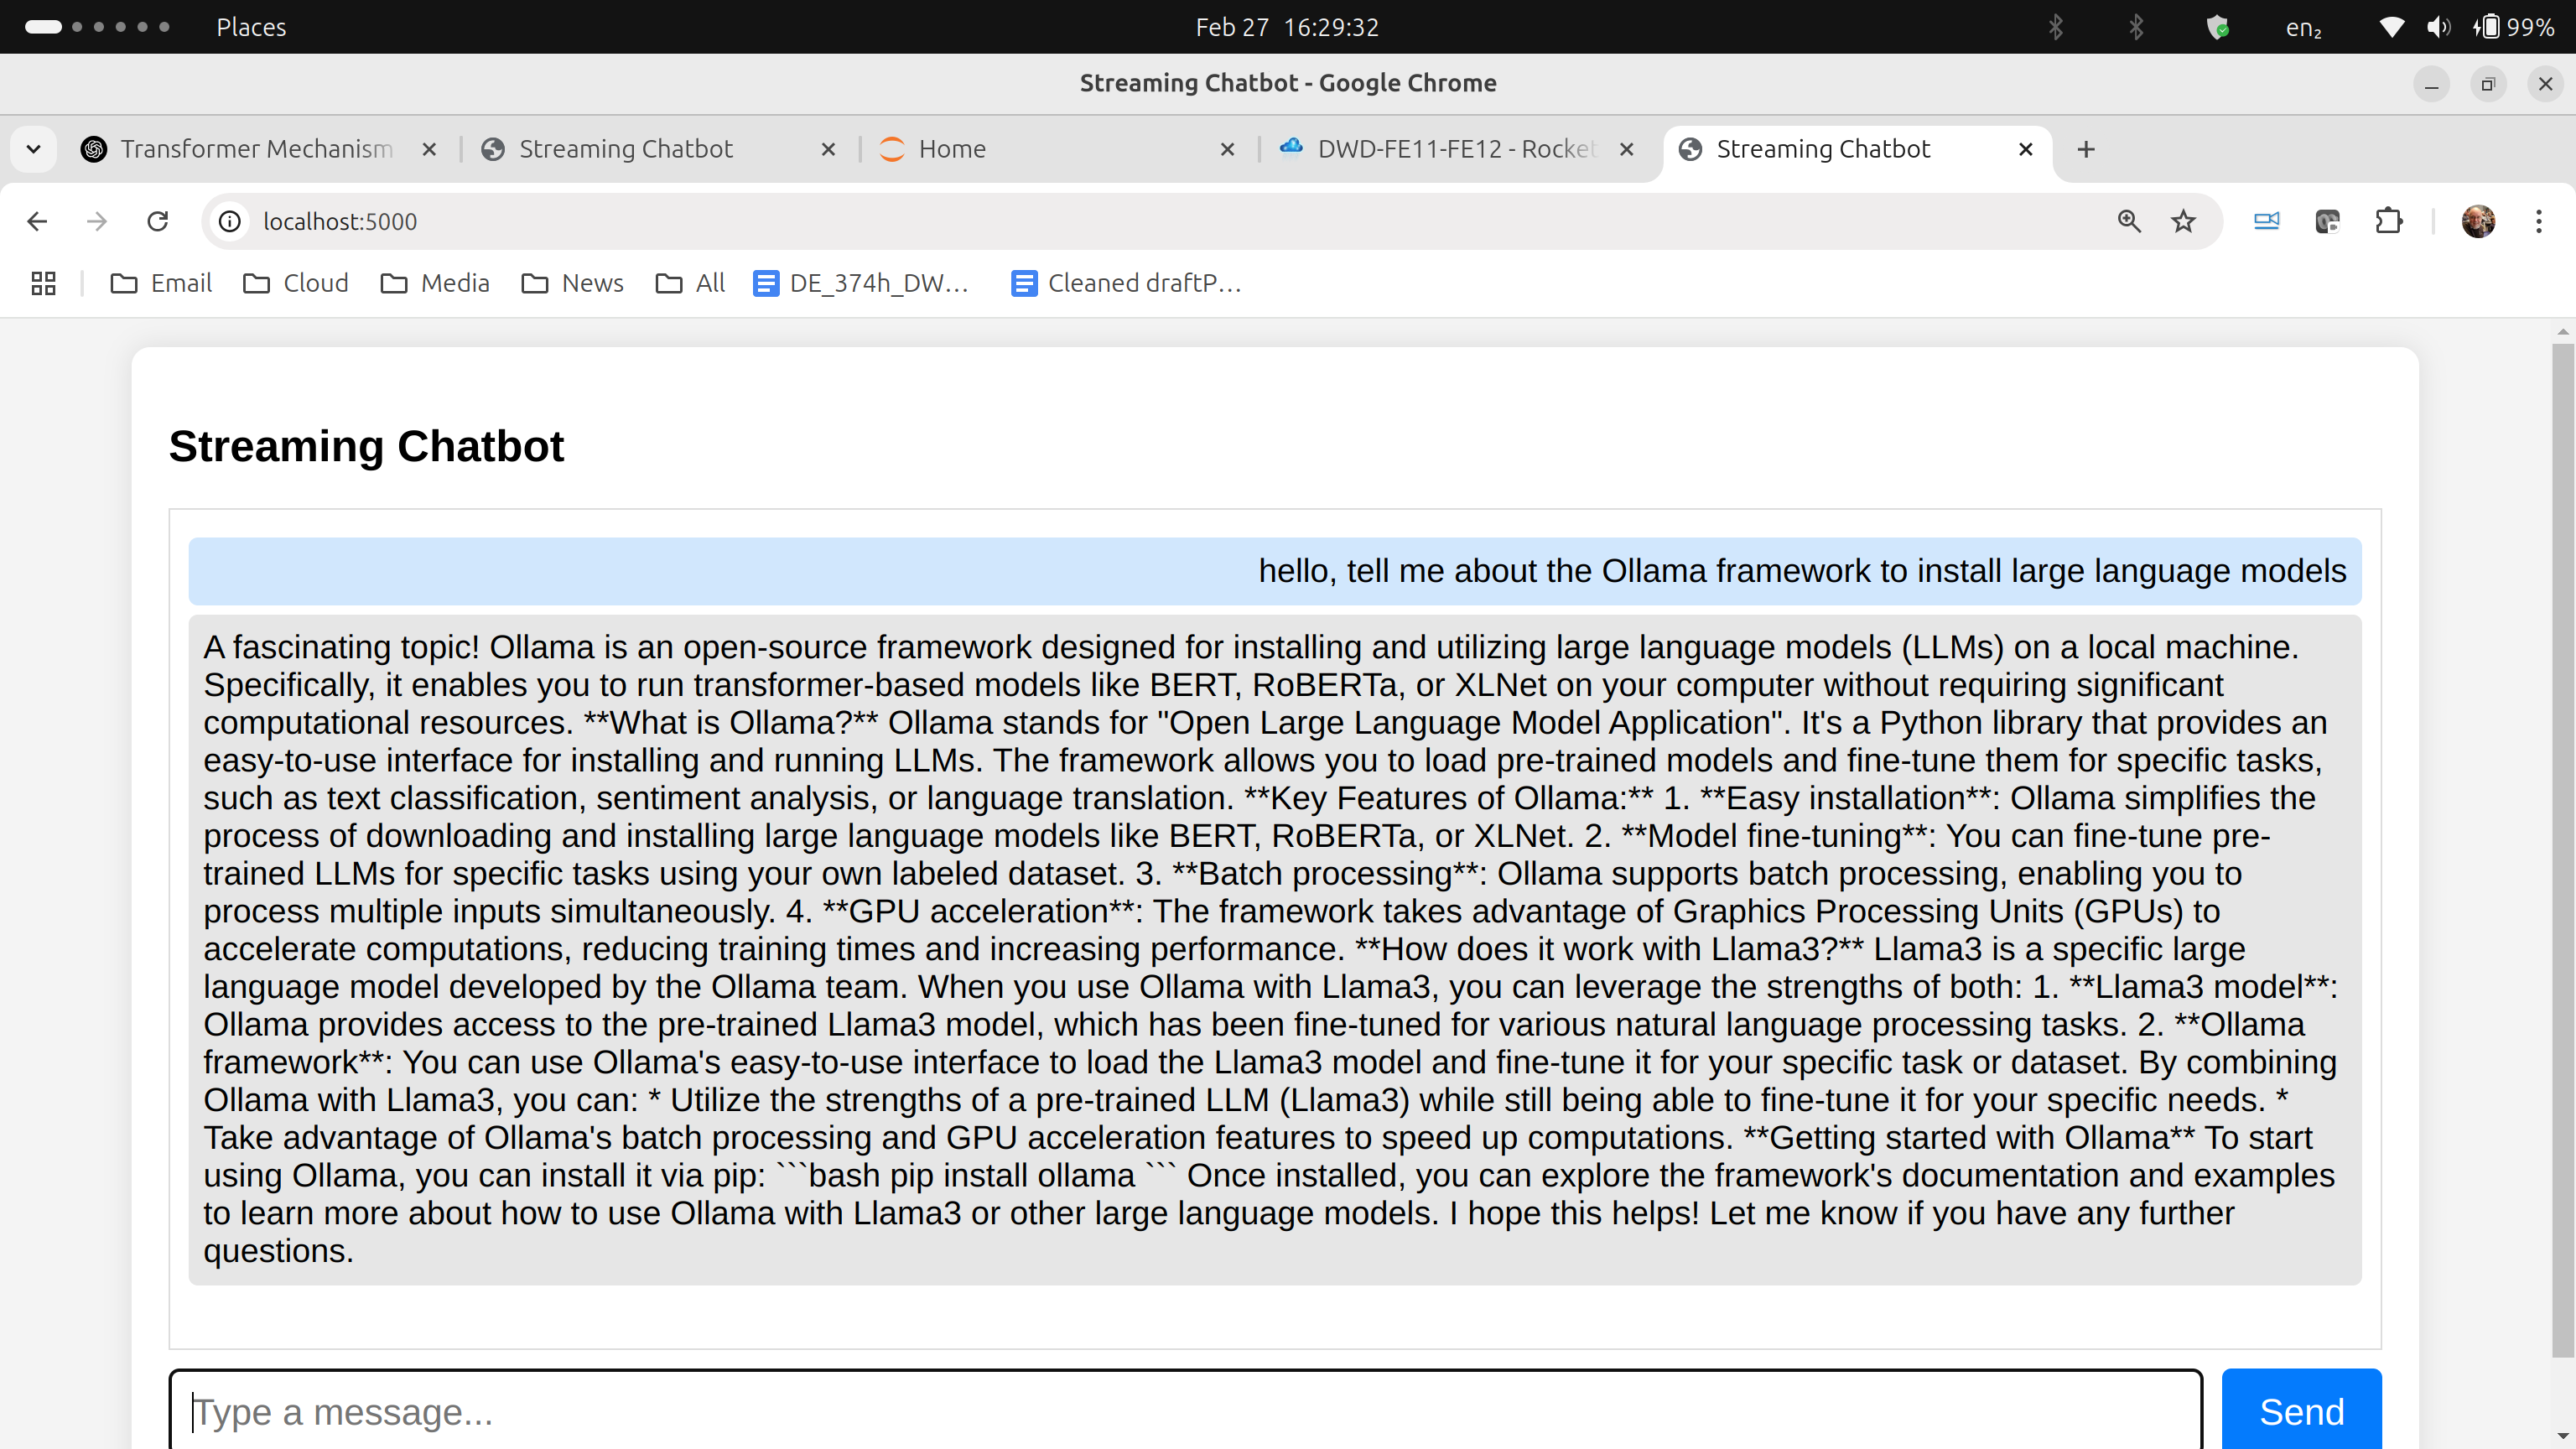
\includegraphics[width=0.8\textwidth]{images/ollama_chatbot.png}
    \caption{Ollama chatbot interface running a local LLM on your laptop, with local UI.}
    \label{fig:ollama_chatbot}
\end{figure}

Once the server is running, you should see output like:

\begin{codeonly}{Server Output}
 * Running on http://127.0.0.1:5000/ (Press CTRL+C to quit)
\end{codeonly}

\subsubsection{Accessing the User Interface}

To interact with the chatbot, open a web browser and go to:

\begin{codeonly}{Accessing the UI}
http://127.0.0.1:5000/
\end{codeonly}

From there, you can enter messages in the input field, and the chatbot will respond accordingly.
This simple local chat UI provides an easy way to interact with Ollama using a web-based interface while maintaining personal chat history.

%==============================================================================
%
%==============================================================================
\subsection{Streaming Responses from Ollama with Markdown Formatting}

In interactive environments such as Jupyter Notebooks or user interfaces (UI), it can be beneficial to stream responses from Ollama in real time while applying Markdown formatting to be able to display e.g. bold words or headings. The following example demonstrates how to achieve this using Python.

The function \texttt{stream\_ollama\_markdown()}:
\begin{itemize}
    \item Sends a request to a locally running Ollama server.
    \item Receives responses in a streaming fashion.
    \item Formats the output dynamically using Markdown to enhance readability.
    \item Updates the output in place without reloading the cell.
\end{itemize}

The function \texttt{format\_markdown()} ensures that:
\begin{itemize}
    \item Capitalized words and model names are bolded for emphasis.
    \item Titles such as "Model Features:" are converted into Markdown headings.
    \item Lists are properly formatted for readability.
\end{itemize}

The demo implementation is given below:

\begin{codeonly}{Streaming Markdown Output from Ollama}
import requests
import json
import re
from IPython.display import display, Markdown, clear_output

def format_markdown(text):
    text = text.replace("\n", "\n\n")
    text = re.sub(r'\b([A-Z][a-z]+(?:\s+[A-Z][a-z]+)*)\b', r'**\1**', text)
    text = re.sub(r'\b([A-Z]{3,})\b', r'**\1**', text)
    return text

def stream_ollama_markdown(prompt, model="llama3"):
    url = "http://localhost:11434/api/generate"
    data = {"model": model, "prompt": prompt, "stream": True}

    response = requests.post(url, json=data, stream=True)
    buffer = ""
    output_display = display(Markdown(""), display_id=True)

    for chunk in response.iter_lines():
        if chunk:
            try:
                data = json.loads(chunk.decode("utf-8"))
                text = data.get("response", "")
                if text:
                    buffer += text
                    clear_output(wait=True)
                    output_display.update(Markdown(format_markdown(buffer)))
            except json.JSONDecodeError:
                pass

    # Final display (in case last chunk isnt shown)
    clear_output(wait=True)
    output_display.update(Markdown(format_markdown(buffer)))
    # No return


# Try it
stream_ollama_markdown("Explain the concept of self-attention in Transformers.")

\end{codeonly}

This method enables seamless streaming of responses from Ollama, allowing for an interactive and visually structured output in Jupyter environments.
We also provide a demo implementation of a streaming interface for your flask based user interface (UI) to Ollama, see \texttt{ollama\_flask\_server\_streaming.py} with the \texttt{index\_stream.html} in the \texttt{templates/} directory. 

%==============================================================================


\subsection{Available Models for Download and Response Speed}

There are more than 150 different LLMs for download and use on Ollama. Here is a selection with some highlighted features. 

\begin{enumerate}
    \item \textbf{DeepSeek-R1 (1.5B – 671B)}  
    A powerful model family covering a wide range of sizes, from small-scale 1.5B to massive 671B parameters, making it flexible for different applications.
    
    \item \textbf{Llama3 (8B, 70B)}  
    One of the most anticipated next-generation models from Meta, optimized for efficiency and capable of handling diverse NLP tasks with strong performance.
    
    \item \textbf{Mistral (7B)}  
    A lightweight model with excellent reasoning capabilities, outperforming many larger models in specific tasks while remaining efficient.
    
    \item \textbf{Qwen2.5 (0.5B – 72B)}  
    Alibaba’s Qwen models are designed for multilingual tasks and reasoning, with a focus on applications requiring high levels of comprehension.
    
    \item \textbf{CodeLlama (7B – 70B)}  
    An LLM specifically optimized for code generation and software development, making it useful for programmers and AI-assisted coding.
    
    \item \textbf{Gemma (2B, 7B)}  
    Google’s Gemma models are efficient and optimized for deployment, designed for responsible AI usage and fine-tuned performance.
    
    \item \textbf{Mixtral (7B, 22B)}  
    A mixture-of-experts (MoE) model that enables highly efficient inference while maintaining competitive accuracy in language tasks.
    
    \item \textbf{Starcoder2 (3B – 15B)}  
    A coding model built for AI-assisted development, capable of understanding and generating code efficiently across multiple programming languages.
    
    \item \textbf{Orca Mini (3B – 70B)}  
    A distilled model trained with advanced reasoning capabilities, making it an excellent option for lightweight yet powerful AI assistants.
    
    \item \textbf{Llava (7B – 34B)}  
    A vision-language model capable of understanding images along with text, useful for applications in multimodal AI tasks like captioning and visual question answering.
\end{enumerate}

\begin{figure}[h]
    \centering
    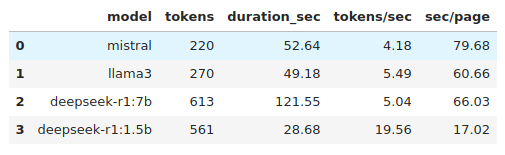
\includegraphics[width=0.8\textwidth]{images/token_per_second.png}
    \caption{Ollama on windows wsl on a regular workstation or laptop. With a light NVIDIA GPU (4GB) speed is about 2.5 times faster. On a linux laptop I got 33 token per second for deepseek-r1:1.5b.}
    \label{fig:ollama_chatbot}
\end{figure}

Large Language Models (LLMs) have become increasingly accessible for local installations, enabling users to process text without relying on cloud services. One crucial performance metric for such models is their response time, typically measured in milliseconds per token.

The speed at which an LLM generates tokens depends on hardware capabilities, model size, and optimization techniques. The DeepSeek-R1:1.5B model on a typical Linux laptop generates one token every 30 milliseconds (ms). The number of tokens generated in a given time frame is given by:
\begin{equation}
    N = \frac{T}{t},
\end{equation}
where:
\begin{itemize}
    \item $N$ is the number of tokens,
    \item $T$ is the total time available (in ms),
    \item $t$ is the time per token (30 ms in this case).
\end{itemize}

For practical scenarios:
\begin{itemize}
    \item In one second ($T = 1000$ ms):
    \begin{equation}
        N = \frac{1000}{30} \approx 33.33 \text{ tokens per second}.
    \end{equation}
    \item In ten seconds ($T = 10000$ ms):
    \begin{equation}
        N = \frac{10000}{30} \approx 333.33 \text{ tokens in ten seconds}.
    \end{equation}
\end{itemize}

To estimate the text length corresponding to these tokens, we assume:
\begin{itemize}
    \item One token typically consists of about 4 characters (including spaces and punctuation).
    \item One token represents approximately 0.75 words in standard English text.
\end{itemize}
Thus, for 333 tokens:
\begin{itemize}
    \item Character count: \( 333 \times 4 = 1332 \) characters.
    \item Word count: \( 333 \times 0.75 \approx 250 \) words.
\end{itemize}
This corresponds to roughly one page of text in a typical document.

The response time of an LLM either online as a service or installed on a local computer significantly influences usability. At 30 ms per token, the DeepSeek-R1:1.5B model can generate around 33 tokens per second or 250 words in ten seconds. Optimizing performance with hardware acceleration (e.g., GPUs, tensor cores) can further improve these figures, making local AI processing a viable alternative to cloud-based models.

\begin{recommendationbox}
Today, medium size LLMs can be run for individual users on a laptop, with acceptable response times for interactive applications. Alternatively and depending on privacy needs the use of platform accounts by AI companies provides faster access to the basic LLM functionality. User services based on either locally or remotely hosted LLM functionality is at hand and can be combined with specific local services and data. 
\end{recommendationbox}
